%%%%%%%%%%%%%%%%%%%%%%%%%%%%%%%%%%%%%%%%%
% University/School Laboratory Report
% LaTeX Template
% Version 3.1 (25/3/14)
%
% This template has been downloaded from:
% http://www.LaTeXTemplates.com
%
% Original author:
% Linux and Unix Users Group at Virginia Tech Wiki 
% (https://vtluug.org/wiki/Example_LaTeX_chem_lab_report)
%
% License:
% CC BY-NC-SA 3.0 (http://creativecommons.org/licenses/by-nc-sa/3.0/)
%
%%%%%%%%%%%%%%%%%%%%%%%%%%%%%%%%%%%%%%%%%

%----------------------------------------------------------------------------------------
%	PACKAGES AND DOCUMENT CONFIGURATIONS
%----------------------------------------------------------------------------------------

\documentclass{article}

\usepackage[version=3]{mhchem} % Package for chemical equation typesetting
\usepackage{siunitx} % Provides the \SI{}{} and \si{} command for typesetting SI units
\usepackage{graphicx} % Required for the inclusion of images
%\usepackage{natbib} % Required to change bibliography style to APA
\usepackage{amsmath} % Required for some math elements 
\usepackage{pifont}
\usepackage{amssymb}
\usepackage{amsthm} 
\usepackage{enumitem}
\setlength\parindent{0pt} % Removes all indentation from paragraphs
\usepackage{subcaption}
\usepackage[toc,page]{appendix}
\usepackage[italian]{babel}

\renewcommand{\appendixtocname}{Appendici}
\renewcommand{\appendixpagename}{Appendici}

%\renewcommand{\labelenumi}{\alph{enumi}.} % Make numbering in the enumerate environment by letter rather than number (e.g. section 6)

%\usepackage{times} % Uncomment to use the Times New Roman font

%----------------------------------------------------------------------------------------
%	DOCUMENT INFORMATION
%----------------------------------------------------------------------------------------

\title{Connettore Publish-Subscribe Content-Based adeguato ad ambiente Mobile per mezzo di politiche adattative } % Title

\author{Stefano \textsc{Agostini} Matricola: 0234240 \\ Paolo \textsc{Salom\'e} Matricola: 0233502 \\ Alessandro \textsc{Valenti} Matricola: 0228709} % Author name

\date{\today} % Date for the report

%\renewcommand{\appendixname}{Appendice}
%\renewcommand{\contentsname}{Indice}

\begin{document}
\selectlanguage{italian}

\maketitle % Insert the title, author and date

\newpage

\tableofcontents

\newpage

%\begin{center}
%\begin{tabular}{l r}
%Date Performed: & January 1, 2012 \\ % Date the experiment was performed
%Partners: & James Smith \\ % Partner names
%& Mary Smith \\
%Instructor: & Professor Smith % Instructor/supervisor
%\end{tabular}
%\end{center}

% If you wish to include an abstract, uncomment the lines below
% \begin{abstract}
% Abstract text
% \end{abstract}

%----------------------------------------------------------------------------------------
%	SECTION 1
%----------------------------------------------------------------------------------------

\section{Introduzione}

Il connettore \textit{Publish-Subscribe} presenta caratteristiche interessanti per sistemi caratterizzati da una elevata dinamicit\'a, grazie all'elevato livello di disaccoppiamento che \'e in grado di garantire tra componenti. I componenti coinvolti nell'interazione, per mezzo del connettore, sono i \textit{produttori} e i \textit{consumatori} di determinati eventi generabili. Un evento \'e caratterizzato dal cosidetto \textit{topic} che rappresenta il suo argomento d'appartenenza al quale un \textit{consumatore} pu\'o sottoscriversi se interessato a tale classe di informazioni; il \textit{produttore} a sua volta pu\'o pubblicare eventi associati ad un determinato \textit{topic}. Nello specifico \'e possibile caratterizzare un determinato evento (dopo averlo associato ad un \textit{topic}) in base al suo contenuto utilizzando la politica del tipo \textit{content-based}. Tale modalit\'a di sottoscrizione viene realizzata specificando un filtro e di conseguenza favorisce la riduzione del carico di eventi recapitati ai \textit{consumatori}. Il connettore realizzato si presta all'utilizzo in ambiente mobile in quanto assicura un alto grado di disaccoppiamento, continuando a garantire uno scambio affidabile di messaggi tra le entit\'a coinvolte. Tuttavia ci siamo posti come obiettivo quello di aggiungere a tale sistema politiche adattative che tengano conto delle limitate risorse energetiche e computazionali a disposizione dei nodi mobili, continuando a garantire uno scambio affidabile di messaggi tra le entit\'a attraverso il connettore.
Intuendo un relazione funzionale tra consumo energetico e traffico generato dal nodo mobile, abbiamo compiuto uno studio statistico per avallare la nostra ipotesi che si \'e rivelato soddisfacente: pertanto abbiamo potuto realizzare un modello matematico finale. 
La nostra politica adattativa ci permette di controllare il tasso di consumo energetico controllando direttamente la frequenza di interazione del nodo mobile con la rete, gestendo, tramite un monitoraggio continuo dello stato della batteria, le risorse limitate del dispositivo. % scrivere in una frase che il nostro sistema implementa mape?

\section{Obiettivi}

L'obiettivo \'e quello di realizzare un connettore \textit{Publish-Subscribe} in modalit\'a \textit{content-based} (basato su \textit{string pattern matching}) ed adattarlo ad ambiente mobile. Nel dettaglio il nostro sistema deve essere costituito da nodi mobili che possono assumere il ruolo di \textit{consumatore o produttore} e dal connettore che deve comporsi delle seguenti entit\'a:

\begin{itemize}
\item{\textit{Event-Service}, il quale si preoccupa di gestire gli eventi generati e di recapitare notifiche}
\item{\textit{Filter-Service}, il quale realizza la modalit\'a di sottoscrizione \textit{content-based}}
\end{itemize}

Si vuole inoltre adattare tale sistema ad ambiente mobile mediante una politica che abbia come scopo quello di monitorare e controllare:

\begin{itemize}
\item{\textit{Il consumo energetico}}
\item{\textit{Il traffico generato} nell'interazione tra nodo mobile e connettore}
\end{itemize}

\section{Architettura generale}

Il sistema si basa fondamentalmente su un'architettura centralizzata. Infatti il connettore \textit{Publish-Subscribe} si compone di un server che svolge sia la funzione di \textit{Event-Service} che la funzione di \textit{Filter-Service}. I client non interagiscono direttamente con il connettore ma scambiano messaggi mediante delle code che implementano il paradigma di interazione \textit{message queueing}. Tale paradigma offre dei vantaggi in termini di disaccoppiamento spaziale e temporale, garantendo la possibilit\'a al client di potersi disattivare o spegnere immediatamente una volta inoltrato un messaggio.
\\
Il server gestisce, tramite una \textit{database non relazionale} distribuito, la persistenza delle informazioni indispensabili per il corretto funzionamento del sistema dal punto di vista dei client, ovvero

\begin{itemize}
\item{\textit{Topic}}
\item{\textit{Sottoscrizioni e Filtri}}
\end{itemize}

I nodi mobili, cos\'i come il server, gestiscono la persistenza in locale di alcune informazioni attraverso un \textit{database relazionale}. Tali informazioni sono i \textit{topic} al momento disponibili nel sistema, le \textit{notifiche} in ingresso, le \textit{sottoscrizioni} effettuate con i relativi \textit{topic e filtri}. Il client attraverso procedure interne effettua, periodicamente,  un'operazione di \textit{pull} sulla coda per poter aggiornare i dati relativi alle notifiche ad esso destinate. Analogamente richiede al server la lista dei \textit{topic} disponibili per aggiornare le sue informazioni locali.\\
Di seguito illustriamo l'architettura attraverso uno schema in \figurename{~\ref{fig:Architettura}}.

\begin{figure}[h]
\begin{center}
\centering
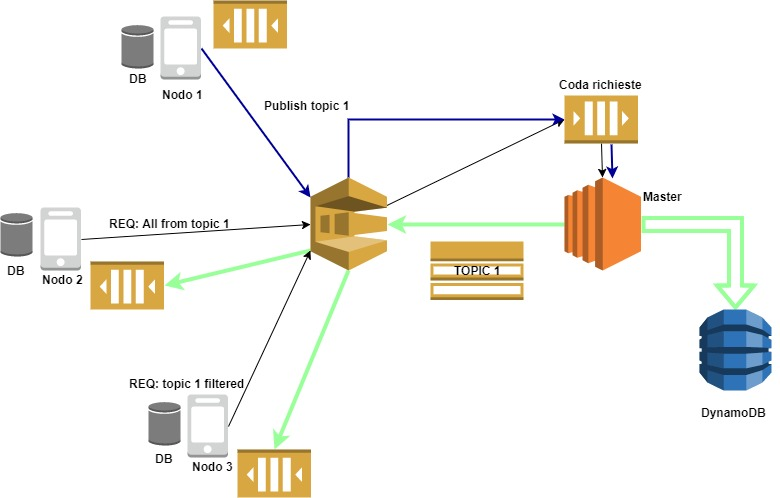
\includegraphics[width=1.25\textwidth]{architettura.jpg} % Include the image placeholder.png
\caption{Architettura}
\label{fig:Architettura}
\end{center}
\end{figure}

\subsection{Servizi Cloud}

Come \textit{Cloud Provider} \'e stato scelto \textit{Amazon AWS}. I servizi utilizzati per l'implementazione del connettore sono:

\begin{itemize}
\item{\textbf{Amazon EC2}: servizio \textit{IaaS} sfruttato per la realizzazione del nodo master che identifica il server dell'architettura. Svolge il ruolo di \textit{Event-Service e Filter-Service} nonch\'e di gestore del \textit{database NoSQL}. Per la comunicazione con i nodi client interagisce con le code del servizio \textit{Amazon SQS}}
\item{\textbf{Amazon SQS}: \'e un servizio di accodamento di messaggi distribuito che disaccoppia completamente i componenti dell'architettura. In tal modo semplifica e riduce i costi del coordinamento dei componenti stessi. Offre un \textit{throughput} elevato e \textit{tunable}, un ordinamento semplificato e distribuzione di tipo \textit{at-least-once}. In generale \'e possibile impostare un algoritmo di \textit{scheduling} dei messaggi: nel nostro caso \'e stato utilizzato l'algoritmo \textit{FIFO}}
\item{\textbf{Amazon DynamoDB}: \'e un servizio di \textit{datastorage} distribuito basato su un \textit{database NoSQL} di tipo \textit{key-value}. \textit{DynamoDB} implementa un sistema di tipo \textit{AP}, disponibilit\'a e tolleranza alle partizioni dei dati, secondo il \textit{CAP Theorem}. L'alto grado di disponibilit\'a ed un accesso di tipo \textit{anywhere} alle informazioni sono due caratteristiche adatte ad un utilizzo in ambiente mobile. Essendo inoltre un database \textit{read-mostly}, ovvero pensato prevalentemente per operazioni di lettura, si adatta perfettamente al nostro sistema, il quale richiede pi\'u letture che scritture.}
\end{itemize}

\subsection{Ambiente Client}
Il nostro sistema \'e pensato per un utilizzo da parte di \textit{client leggeri} con sistema operativo \textit{Android}. \textit{Android} \'e un sistema operativo per dispositivi mobili sviluppato da \textit{Google Inc.} e basato sul kernel \textit{Linux}. Le applicazioni che vengono eseguite sulle piattaforme \textit{Android} sono scritte prevalentemente in linguaggio \textit{Java}, come nel nostro caso. L'applicazione \textit{client} interagisce con un \textit{database relazionale} interno di tipo \textit{SQLite}.

\subsection{Ambiente Server}
Sfruttando il servizio \textit{IaaS di Amazon EC2}, \'e stato possibile scegliere il sistema operativo del server e le caratteristiche della macchina \textit{host}. In particolare abbiamo scelto un'istanza \textit{t2.micro} dotata di una \textit{virtual cpu}, \textit{1 GB di ram} e \textit{8 GB di storage}. \'E stato scelto come sistema operativo \textit{Linux Ubuntu Server v.16.04 LTS}. La scelta di tale sistema operativo \'e da ricondurre alla semplicit\'a di installazione di componenti aggiuntivi e alla sua versatilit\'a.

\subsection{Interazione dei componenti}
Per promuovere la comunicazione tra i client ed il server, disaccoppiandoli, \'e stato scelto di utilizzare diverse code \textit{SQS}, partizionandone i compiti. In particolare vengono generate tre code fisse per richiedere l'esecuzione delle operazioni fondamentali di un sistema \textit{Publish-Subscribe} al  server:

\begin{itemize}
\item{\textbf{Creation Queue}: i client scrivono su questa coda per richiedere al server la creazione di un determinato \textit{topic}}
\item{\textbf{Notification Queue}: i client scrivono su questa coda per pubblicare una notifica su un determinato \textit{topic}}
\item{\textbf{Subscription Queue}: i client scrivono su questa coda per sottoscriversi in modalit\'a \textit{content-based} ad un determinato \textit{topic} oppure annullare una sottoscrizione precedentemente effettuata}
\end{itemize}

Ogni messaggio proveniente dai nodi mobili raggiunge il server per mezzo delle tre code fisse sopra descritte (come si nota in \figurename{~\ref{fig:Architettura}}). Il server elabora i messaggi in ingresso ed aggiorna le informazioni riguardanti i \textit{topic} e le sottoscrizioni nell'istanza di \textit{DynamoDB}.
\\
Per la ricezione di messaggi ogni client ha a disposizione una coda dedicata, la quale viene creata al momento dell'ingresso del nodo nel sistema ed \'e utilizzata per la ricezione dei messaggi di notifica.
\\
Infine il database \textit{SQLite}, presente in ogni client, \'e utilizzato per tenere traccia dei \textit{topic} presenti al momento nell'istanza di \textit{DynamoDB} e per memorizzare le notifiche ricevute.

\section{Implementazione}

\subsection{Server}
Abbiamo scelto di utilizzare lato server la piattaforma \textit{event-driven Node.js} per motivi di immediatezza, versatilit\'a  ed efficienza. Tale piattaforma supporta il linguaggio di programmazione \textit{Javascript}, linguaggio di scripting orientato agli oggetti e agli eventi. L'efficienza di \textit{Node.js} \'e legata al suo modello di \textit{networking}, ossia \textit{I/O event-driven}. La piattaforma richiede al sistema operativo di ricevere notifiche al verificarsi di determinati eventi e rimane in modalit\'a \textit{sleep} fino alla ricezione della notifica stessa, in corrispondenza della quale avvia l'esecuzione di una funzione di \textit{callback} di risposta. Tale modello di \textit{networking} si rivela efficiente nella gestione di un elevato traffico di rete, come potrebbe accadere nel caso del nostro sistema.
\\
Di seguito ci apprestiamo a descrivere puntualmente l'implementazione dei componenti server.

\subsubsection{Formato \textit{JSON} dei messaggi scambiati}

I messaggi diretti da client a server possono essere di tre tipi (un tipo per coda):

\begin{itemize}

\item{\textbf{Crezione-rimozione di un topic}:}

\begin{tabular}{ll}
\{\\
	   \hspace{10mm} \textbf{"type"}: string, // "CREATE" or "DELETE"\\
              \hspace{10mm} \textbf{"userID"}: string, // macaddress\\
              \hspace{10mm} \textbf{"topicName"}: string
\\
\}
\end{tabular}

\item{\textbf{Sottoscrizione-Cancellazione}:}

\begin{tabular}{ll}
\{\\	   
            \hspace{10mm} \textbf{"type"}: string, // "SUB" or "UNSUB" or "UNSUBALL"\\
            \hspace{10mm} \textbf{"userID"}: string, // macaddress\\
            \hspace{10mm} \textbf{"topicName"}: string,\\
            \hspace{10mm} \textbf{"filter"}: string 
\\
\}
\end{tabular}

\item{\textbf{Pubblicazione di notifiche}:}

\begin{tabular}{ll}
\{\\	   
           \hspace{10mm} \textbf{"userID"}: string, // macaddress\\
           \hspace{10mm} \textbf{"topicName"}: string,\\
           \hspace{10mm} \textbf{"messageBody"}: string
\\
\}
\end{tabular}

\end{itemize}

I messaggi di notifica elaborati dal server e destinati alle code dedicate dei client hanno il seguente formato:
\\\\
\begin{tabular}{ll}
\{\\	   
           \hspace{10mm} \textbf{"topicName"}: string, \\
           \hspace{10mm} \textbf{"messageBody"}: string
\\
\}
\end{tabular}

\subsubsection{AWS SDK}
\textit{Amazon AWS} mette a disposizione delle librerie ai programmatori per consentirgli di interagire e accedere ai servizi \textit{Cloud} da codice. In particolare \textit{AWS} supporta anche \textit{Javascript} con le proprie \textit{SDK} (\textit{Software Development Kit}). Sono state utilizzate le \textit{API AWS SDK} relative ai servizi \textit{SQS e DynamoDB} ed estese per mezzo di due librerie: \textit{sqs\_api.js e dynamo\_api.js}.\\

\textbf{sqs\_api.js}
\begin{itemize}
\item{\textit{create\_queue}: crea una coda identificata dall'attributo \textit{QueueNamePrefix} (parametro della funzione) se non esiste. Questa funzione viene utilizzata sia per la creazione delle tre code fisse che di quelle dedicate ai singoli nodi client.}
\item{\textit{write\_queue}: scrive un messaggio nella coda specificata (messaggio e nome della coda entrambi parametri della funzione). Per risalire alla coda, ricava il suo \textit{URL} mediante l'\textit{API SDK getQueueUrl} utilizzando il suo nome. Se il recupero va a buon fine, viene inviato il messaggio sulla coda invocando \textit{l'API SDK sendMessage}.}
\item{\textit{read\_queue}: legge i messaggi presenti nella coda di cui \'e specificato il nome (parametro della funzione). Ricava lo \textit{URL} della coda mediante l'\textit{API SDK getQueueUrl} alla quale passa il nome come argomento. Se la \textit{getQueueUrl} va a buon fine, vengono recuperati i messaggi presenti nella coda selezionata grazie all'\textit{API SDK receiveMessage}. Nella \textit{callback} della \textit{receiveMessage} viene generato un nuovo processo che resta in attesa della comunicazione dei messaggi da parte del processo padre. Quest'ultimo invia i messaggi letti dalla coda al processo figlio sfruttando la funzione \textit{send} dell'\textit{IPC di Node.js}.  In ricezione, il processo figlio (definito come \textit{consumer}, i cui dettagli sono nella sezione 4.1.4) elabora i messaggi e termina. Tutti i messaggi letti dalla coda vengono eliminati dalla stessa attraverso la funzione \textit{delete\_messages} che ci apprestiamo a descrivere.}
\item{\textit{delete\_messages}: prende come parametri lo \textit{URL} della coda e la lista delle \textit{entries} lette, oggetti che seguono un formato specificato dagli standard \textit{AWS SDK}. Per l'eliminazione viene invocata l'\textit{API SDK deleteMessageBatch}, la quale permette la cancellazione di \textit{batch} interi di messaggi.}
\end{itemize}

\textbf{dynamo\_api.js}
\begin{itemize}
\item{\textit{creation\_table}: prende come parametro il nome della tabella da creare se non esiste (supporta la creazione delle tabelle \textit{Topic e Subscription}). Definisce il formato della tabella per la sua creazione per mezzo dell'\textit{API SDK createTable}. La tabella \textit{Topic} ha come chiave il \textit{topicName} (\textit{string}) che ricopre il ruolo di \textit{partition key}. Invece la tabella \textit{Subscription} ha come chiave la coppia \textit{(topicName, userID)} (entrambe stringhe) e la prima ha il ruolo di \textit{partition key} mentre la seconda quello di \textit{sort key}.}
\item{\textit{create\_topic}: prende come parametri il \textit{topicName} e lo \textit{user\_id} (creatore del \textit{topic}). Utilizza l'\textit{API SDK get} e, se il \textit{topic} non \'e presente nella tabella \textit{Topic}, crea un nuovo \textit{item} e lo salva usando l'\textit{API SDK put}.}
\item{\textit{delete\_topic}: prende come parametri il \textit{topic\_name} e lo \textit{user\_id} (identificativo del client che ha richiesto al server di rimuovere il \textit{topic}). Recupera, mediante l'\textit{API SDK get}, il \textit{topic} dalla tabella e controlla se l'\textit{id} del creatore coincide con l'\textit{id} del client richiedente. In caso affermativo rimuove l'\textit{item} dalla tabella usando l'\textit{API SDK delete}.}
\item{\textit{create\_subscription}: prende come parametri \textit{topic\_name, user\_id} e \textit{filter}. Controlla l'esistenza del \textit{topic} nella tabella \textit{Topic}. Se \'e verificata scrive nella tabella \textit{Subscription} il nuovo \textit{item}, con chiave \textit{(topic\_name, user\_id)}.}
\item{\textit{delete\_subscription}: prende come parametri \textit{topic\_name} e \textit{user\_id}. Effettua la cancellazione dalla tabella \textit{Subscription} dell'\textit{item} con chiave \textit{(topic\_name, user\_id)}, usando l'\textit{API SDK delete}.}
\item{\textit{scan\_all\_topics}: utilizza l'\textit{API SDK scan} per estrarre la lista dei \textit{topic} al momento presenti nel sistema.}
\item{\textit{send\_notification}: prende come parametri \textit{topic\_name} e \textit{message\_body} (rispettivamente il \textit{topic} e il messaggio inviato dal client che vuole effettuare una \textit{publish} su di esso). Effettua una \textit{query} sulla tabella \textit{Subscription}, tramite l'\textit{API SDK query}, specificando il \textit{topic\_name}. Il risultato delle \textit{query} \'e una lista di coppie \textit{(user\_id, filter)}, ognuna delle quali rappresenta un sottoscritto al \textit{topic} ed il relativo filtro. Per ogni \textit{item} della lista viene controllata l'occorrenza del suo filtro all'interno del \textit{message\_body}, ed in caso fosse verificata viene inoltrata la notifica alla coda dedicata del client mediante la funzione \textit{write\_queue} della libreria \textit{sqs\_api.js}.}
\end{itemize}

\subsubsection{\textit{Readers}}
I tre processi \textit{Readers} si occupano di leggere periodicamente dalle tre code fisse \textit{Creation Queue}, \textit{Notification Queue} e \textit{Subscription Queue}. Tali processi sono continuamente in esecuzione e sfruttano la funzione \textit{polling} del modulo \textit{polling.js}, la quale legge periodicamente dalla coda specificata, passata come argomento, mediante la funzione \textit{read\_queue} della libreria \textit{sqs\_api}. Nel caso in esame \'e stato scelto come intervallo di lettura un tempo pari a \textit{5000 millisec}.

\subsubsection{\textit{Consumer e Updaters}}
Ogni processo di tipo \textit{Reader}, alla lettura dei messaggi dalla sua coda (tramite la funzione di lettura \textit{read\_queue} del modulo \textit{sqs\_api}), crea un processo di tipo \textit{Consumer} invocando una \textit{fork} con argomento il modulo \textit{consumer.js} e successivamente gli invia i messaggi letti tramite la funzione \textit{send} dell'\textit{IPC} di \textit{Node.js}. Ogni \textit{Reader} invia al processo \textit{Consumer} un messaggio che segue il seguente formato:
\\\\
\begin{tabular}{ll}
\{\\	   
           \hspace{10mm} data: data\_read.Messages, // Lista dei messaggi letti dalla coda \\
           \hspace{10mm} queue: queue\_name // Nome della coda di lettura
\\
\}
\end{tabular}
\\\\
In tal modo il processo \textit{Consumer} pu\'o distinguerne la coda di appartenenza per delegare al corrispondente \textit{Updater} la gestione dei dati letti (\textit{data\_read.Messages}). Gli \textit{Updaters} sono tre funzioni, ognuna implementata nel suo modulo:

\begin{itemize}
\item{\textit{notification\_updater}: funzione eseguita quando \textit{queue = notificationQueue}. Per ogni messaggio in \textit{data\_read.Messages} invoca la funzione \textit{send\_notification} della libreria \textit{dynamo\_api}.}
\item{\textit{subscription\_updater}: funzione eseguita quando \textit{queue = subscriptionQueue}. Per ogni messaggio, in base al tipo (\textit{SUB o UNSUB}), invoca la funzione \textit{create\_subscription} o \textit{delete\_subscription}, entrambe appartenenti alla libreria \textit{dynamo\_api}.}
\item{\textit{topic\_updater}: funzione eseguita quando \textit{queue = creationQueue}. Per ogni messaggio, in base al tipo (\textit{CREATE o DELETE}), invoca la funzione \textit{create\_topic} o \textit{delete\_topic}, entrambe appartenenti alla libreria \textit{dynamo\_api}.}
\end{itemize}

Al termine della gestione dei messaggi letti il processo \textit{Consumer} termina.

\subsubsection{\textit{Server Http e Routes}}
Al fine di separare le \textit{routes} dal server \textit{http} \'e stato utilizzato il \textit{framework Express.js}. Nel modulo \textit{routes.js} \'e disponibille un \textit{endpoint} per rispondere a richieste \textit{http} di tipo \textit{get}, il quale invoca la funzione \textit{scan\_all\_topics di dinamo\_api.js} per restituire al client richiedente la lista di tutti i \textit{topic} presenti nel sistema. Il \textit{Server http} \'e un processo che utilizza le \textit{routes} e rimane in ascolto sulla porta \textit{8080}.

\subsubsection{\textit{Main}}
Il modulo \textit{main.js} crea le tre code fisse del sistema invocando la funzione \textit{create\_queue} di \textit{sqs\_api} e le tabelle \textit{Subscription e Topic} tramite la funzione \textit{creation\_table} di \textit{dinamo\_api}. Infine, per mezzo di \textit{fork}, avvia i quattro processi stabili del sistema: i tre \textit{Readers} e il \textit{Server http}. \\
In \figurename{~\ref{fig:Processi}} troviamo lo schema dei processi attivi nel server: \'e possibile osservare che vi sono quattro processi sempre attivi e diversi processi temporanei che eventualmente si attivano con cadenza temporale di \textit{5 sec}.

\begin{figure}[h!]
\begin{center}
\centering
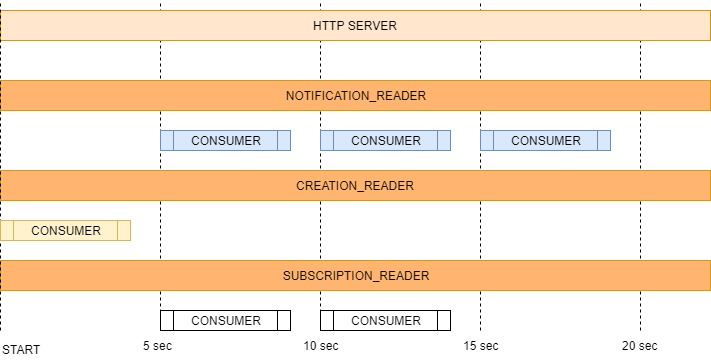
\includegraphics[width=1.1\textwidth]{stableprocess.jpg} % Include the image placeholder.png
\caption{Processi}
\label{fig:Processi}
\end{center}
\end{figure}

\subsection{Client}
L'applicazione lato client \'e stata realizzata in modo tale da potersi adattare secondo due modalit\'a in risposta al consumo attuale di batteria:
\begin{itemize}
\item{\textbf{modalit\'a dinamica}: il client \'e un sistema \textit{self-adaptive}, ovvero in base al livello attuale di batteria del dispositivo modula la frequenza di interazione con la sua coda dedicata, limitando l'utilizzo della scheda di rete. Implementa il \textit{feedback-control-loop} di \textit{MAPE-K}. }
\item{\textbf{modalit\'a statica}: l'utente che utilizza l'applicazione pu\'o impostare una politica di risparmio energetico a priori, con la quale si limita la luminosit\'a dello schermo del dispositivo. }
\end{itemize}
Poich\'e di maggiore interesse, \'e stata dimostrata l'efficacia della politica in modalit\'a dinamica e nel seguito della trattazione verranno mostrati i test ed il modello matematico finale corrispondente.

\subsubsection{\textit{Util}}
Questa classe contiene diversi metodi che si possono raggruppare in categorie:
\begin{itemize}
\item{Metodo per accedere ai servizi di \textit{AWS SQS}(\textit{getProperty}).}
\item{Metodo per rilevare il livello di batteria attuale del dispositivo (\textit{getBatteryLevel}). }
\item{Metodi per convertire nel corretto formato i messaggi destinati al connettore (\textit{createDelete,subUnsub,publish}), attraverso le tre code fisse precedentemente descritte.}
\item{Metodo per recuperare la lista dei \textit{Topic} presenti attualmente nel sistema (\textit{getTopicList}). Contatta l'endpoint del server (\textit{allTopics}) ed eventualmente compatta i messaggi di risposta.}
\end{itemize}
\subsubsection{\textit{DBHelper}}
Questa classe estende \textit{SQLiteOpenHelper} e fornisce i metodi \textit{CRUD} sulle tabelle del \textit{DB} locale. Le tabelle sono le seguenti:
\begin{itemize}
\item \textbf{Filtered}: \'e la tabella contenente le notifiche destinate all'utente ed ha il seguente schema:
	\begin{itemize}
	\item	\textit{id}: id della notifica;
	\item 	\textit{date}: data di ricezione dalla coda;
	\item	\textit{topic}: \textit{Topic} di appartenenza;
	\item	\textit{content}: contenuto della notifica.
	\end{itemize}
\item \textbf{Topic}: \'e la tabella contenente tutti i \textit{Topic} aggiornati all'ultima richiesta al server ed ha il seguente schema:
	\begin{itemize}
	\item	\textit{id}: id del \textit{Topic};
	\item	\textit{name}: nome del \textit{Topic}.
	\end{itemize}
\item \textbf{TopicFiltered}: \'e la tabella contenente tutti i \textit{Topic} a cui l'utente si \'e sottoscritto con il filtro associato ed ha il seguente schema:
	\begin{itemize}
	\item	\textit{id}: id del \textit{Topic};
	\item	\textit{name}: nome del \textit{Topic};
	\item 	\textit{filter}: filtro di sottoscrizione sul topic.
	\end{itemize}
\end{itemize}
\subsubsection{\textit{AWSSimpleQueueServiceUtil}}
Questa classe implementa dei metodi per accedere ai servizi \textit{AWS SQS} mediante l'utilizzo delle \textit{API AWS SDK}. Tali metodi sono i seguenti:
\begin{itemize}
\item	{\textit{createQueue}: prende come argomento il nome della coda e la crea utilizzando l'\textit{API AWS SDK createQueue}. Restituisce infine l'\textit{URL} della coda.}
\item	{\textit{getQueueUrl}: restituisce l'\textit{URL} della coda il cui nome \'e passato come argomento. Usa l'\textit{API AWS SDK getQueueUrl}.}
\item	{\textit{sendMessageToQueue}: invia un messaggio sulla coda (una delle tre code fisse) identificata dal suo \textit{URL}, passati entrambi come argomento.  Usa l'\textit{API AWS SDK sendMessage}. }
\item	{\textit{getMessagesFromQueue}: specificato l'\textit{URL} della coda dedicata del client, legge i messaggi presenti nella stessa usando l'\textit{API AWS SDK receiveMessage}. Infine restituisce una lista.}
\item 	{\textit{deleteMessageFromQueue}: cancella un messaggio dalla coda dedicata identificata dal suo \textit{URL}, entrambi passati come argomento. Usa l'\textit{API AWS SDK deleteMessage}.}
\end{itemize}
\subsubsection{\textit{Fragment}}
Un \textit{Fragment} rappresenta un ambiente oppure una porzione dell'interfaccia in una Activity. Si pu\'o pensare a un \textit{Fragment} come sezione modulare di un'attivit\'a che ha un proprio ciclo di vita, riceve i propri eventi di input e che \'e possibile aggiungere o rimuovere mentre l'attivit\'a \'e in esecuzione. 
\'E possibile combinarne diversi in una singola \textit{activity} per costruire una \textit{multi-pane UI}, e questo \'e quello che ci ha spinti all'utilizzo degli stessi.
\\Nella fase di inizializzazione dei \textit{Fragment} vengono eseguiti gli \textit{AsyncTask}. \\L'\textit{AsyncTask} consente l'uso corretto e semplice del \textit{thread UI}. Tale classe permette di eseguire operazioni in background e pubblicare risultati sul thread dell'interfaccia utente senza dover manipolare i \textit{threads} e/o \textit{handlers}. Un \textit{AsyncTask} ha il compito di eseguire una porzione di codice su un \textit{thread} in background, il cui risultato viene pubblicato sul \textit{thread UI}.

Nella nostra applicazione sono presenti quattro tipologie di \textit{Fragment}:
\begin{itemize}
\item \textbf{ReadFragment}: consente all'utente di leggere i messaggi presenti nel \textit{DB} del dispositivo mobile raggruppati per \textit{Topic}. All'avvio viene invocato un \textit{AsyncTask} per popolare una \textit{listView} (presente sul layout \textit{activity\_Read}) contenente tutti i \textit{Topic} a cui l'utente si \'e sottoscritto. All'interno dell'\textit{Async-Task}, per recuperare i dati dal \textit{DB} viene invocato il metodo \textit{getAllTopicFilter} della classe \textit{DBHelper}.
Alla selezione di un \textit{item} della lista viene eseguito il secondo \textit{AsyncTask}, il quale popoler\'a nuovamente la \textit{listView} con le notifiche presenti nel \textit{DB} relative a quel \textit{Topic}.
All'interno dell'\textit{AsyncTask}, per recuperare le notifiche dal \textit{DB}, relative al \textit{Topic} selezionato, viene invocato il metodo \textit{getFilteredMessageByTopicName} della classe \textit{DBHelper}.
\item \textbf{WriteFragment}: consente all'utente di pubblicare notifiche sui \textit{Topic} attualmente esistenti o di crearne di nuovi. All'avvio viene invocato un \textit{AsyncTask} per popolare una \textit{listView} (presente sul layout \textit{activity\_write}) contenente tutti i \textit{Topic} attualmente nel sistema. All'interno dell'\textit{AsyncTask} viene invocato il metodo \textit{getTopicList}, fornito dalla classe \textit{Util}, per contattare il server con il fine di ottenere la lista dei \textit{Topic} presenti nel sistema. Ogni \textit{item} della \textit{listView} pu\'o essere selezionato per inviare una notifica su quel \textit{Topic}: questa fase richiede l'interazione con l'utente, il quale dovr\'a scrivere il testo della notifica per poi confermarne l'invio. La notifica viene formattata utilizzando il metodo \textit{publish} della classe \textit{Util}, ed inviata con l'utilizzo dell' \textit{API AWS SDK sendMessageToQueue} specificando la coda \textit{notificationQueue} in quest'ultima. 
\\La creazione di nuovi \textit{Topic} \'e possibile in pochi passi:
\begin{itemize}
\item	L'utente seleziona un tasto presente sull'\textit{activity\_write};
\item	compare a schermo una finestra di dialogo in cui inserire il nome del nuovo \textit{Topic};
\item 	se si conferma l'operazione, viene inviata una richiesta di creazione \textit{Topic} al server con l'utilizzo dell'\textit{API AWS SDK sendMessageToQueue} verso la coda \textit{creationQueue}. La creazione del \textit{Topic} \'e cos\'i 		demandata al server che gestisce la richiesta come spiegato in precedenza.
\end{itemize}

\item \textbf{SetFilterFragment}: consente all'utente di sottoscriversi ad i \textit{Topic} attualmente esistenti. All'avvio viene invocato un \textit{AsyncTask} per popolare una \textit{gridView} (presente sul layout \textit{activity\_set\_filter}) contenente per ogni \textit{Topic} attualmente nel sistema il filtro di sottoscrizione associato. All'interno dell'\textit{AsyncTask} si eseguono i seguenti passi:
\begin{itemize}
\item 	Viene invocato il metodo \textit{getTopicList}, fornito dalla classe \textit{Util}, per contattare il server con il fine di ottenere la lista dei \textit{Topic} presenti nel sistema;
\item	vengono salvati gli eventuali nuovi \textit{Topic} all'interno del \textit{DB}, utilizzando il metodo \textit{insertNotExistTableTopic} della classe \textit{DBHelper};
\item	si recupera la lista di tutti i \textit{Topic}, ciascuno con l'eventuale filtro associato.
\item si popola la \textit{gridView}.
\end{itemize}
L'utente pu\'o selezionare ciascun \textit{item} della griglia per cambiare il filtro corrispondente a quel \textit{Topic} o per richiedere una nuova sottoscrizione. Se si conferma l'operazione, viene inviata una richiesta di sottoscrizione \textit{Topic} al server con l'utilizzo dell'\textit{API AWS SDK sendMessageToQueue} verso la coda \textit{subscriptonQueue}.
\item \textbf{SettingsFragment}: consente all'utente di impostare l'applicazione in modalit\'a risparmio energetico, la quale non far\'a altro che impostare la luminosit\'a dello schermo ad un valore fissato. L'utente pu\'o attivare o meno questa modalit\'a grazie ad uno \textit{Switch} presente nell'\textit{activity\_settings}.
\end{itemize}

\subsubsection{\textit{MainActivity}}
La \textit{MainActivity} contiene tutti i controlli utili per la navigazione all'interno delle sezioni dell'applicazione (ossia quelle di pubblicazione notifiche, sottoscrizione \textit{Topic}, lettura notifiche) e passa quindi il controllo al \textit{Fragment} corrispondente alla sezione prescelta. Inoltre \'e presente un \textit{AsyncTask} con il compito di prelevare le notifiche in arrivo, leggendole dalla coda dedicata con l'utilizzo dell'\textit{API AWS SDK getMessageFromQueue}; tale coda viene creata utilizzando un \textit{Android ID} ovvero un codice identificativo unico per ogni sistema operativo installato su dispositivo. L'operazione di \textit{pull} \'e effettuata periodicamente con frequenza di \textit{pull} dipendente dal livello corrente della batteria del dispositivo:
\begin{itemize}
\item   75\% \textless  Livello batteria \textless= 100\% \ding{226} 1 pull ogni secondo
\item	50\% \textless  Livello batteria \textless= 75\%  \ding{226} 1 pull ogni 5 secondi
\item	0\% \textless  Livello batteria \textless= 50\%  \ding{226} 1 pull ogni 30 secondi
\end{itemize}
 
Questa scelta \'e motivata dai risultati ottenuti dallo studio sulla relazione funzionale che esiste tra frequenza di \textit{pull} (e quindi frequenza di utilizzo della scheda di rete) e consumo della batteria. Nel prossimo capitolo viene illustrato l'esito di tale indagine.

\section{Politica adattativa}

\subsection{Oggetto dell'analisi}
La natura limitata inerente ai dispositivi mobili impone al progettista di sistemi informatici di condurre la ricerca di una politica adattativa che preservi le loro risorse computazionali e/o energetiche e/o di memoria, inevitabilmente finite e degradabili. Non possono pertanto essere trascurate, nell'atto della progettazione e realizzazione di un sistema informatico, le differenze sostanziali che intercorrono tra nodi fissi e nodi mobili in termini di \textit{abbondanza} di risorse fisiche ed energetiche: conseguenza il rapido degrado e la mala gestione delle stesse. 
\\
L'idea \'e quella di identificare una risorsa misurabile del dispositivo mobile, finita e degradabile, e di tentare di risalire ad una sua relazione funzionale con una variabile (indipendente) direttamente controllabile. Una tale relazione tra le due grandezze permetterebbe di limitare e gestire il deterioramento della risorsa del dispositivo, modificando semplicemente il valore della variabile indipendente (e controllabile). In sintesi si cerca una relazione del tipo: 
\\\\
\{\textit{f}(\(\theta\)), \(\theta\) \(\in\) \textit{K}\}
\\\\
Laddove:
\begin{itemize}
\item{\textit{f}(\(\theta\)) \'e la misura della risorsa del dispositivo da gestire}
\item{\(\theta\) \'e la variabile indipendente e controllabile}
\item{\textit{K} \'e l'insieme di definizione della variabile indipendente e controllabile}
\end{itemize}

Nel caso in esame \'e stato deciso di gestire e limitare la velocit\'a di scarica della batteria del dispositivo: ovvero \textit{f}(\(\theta\)) \'e \textbf{la variazione del livello di carica della batteria nel tempo}. Analizzando il sistema \'e risultata evidente una relazione attiva tra tale misura e la \textbf{frequenza di pull alla coda dedicata} al client. Quest'ultima assume il ruolo di variabile indipendente e controllabile \(\theta\) del modello matematico sopra esposto. 
\\
Per definire il modello matematico occorre risalire all'entit\'a della relazione funzionale \textbf{\textit{f}} che lega le due grandezze. A tal proposito viene utilizzato lo strumento matematico della \textbf{\textit{regressione}}, che richiede di effettuare misure della grandezza in esame.
\\
Il modello matematico viene realizzato seguendo tre fasi:

\begin{enumerate}
\item{Identificazione della relazione funzionale esistente tra il \textit{livello della batteria \textit{f}\textsubscript{p}(\textit{t})} ed il \textit{tempo t}, fissata una certa \textit{frequenza di pull p}.}
\item{Calcolo della derivata rispetto al tempo di \textit{f}\textsubscript{p}(\textit{t}) ovvero \(\frac{df\textsubscript{p}(\textit{t})}{dt}\), che rappresenta la \textit{velocit\'a media di scarica} della batteria del dispositivo fissata una certa \textit{frequenza di pull p}. La derivata rispetto al tempo del livello di batteria \'e la grandezza che si vuole limitare e gestire.}
\item{Identificazione della relazione funzionale esistente tra la \textit{velocit\'a media di scarica \(\frac{df\textsubscript{p}(\textit{t})}{dt}\)} e la corrispondente \textit{frequenza di pull p}.}
\end{enumerate} 

\subsection{Test e risultati}

Per effettuare le misurazioni della grandezza in esame, \'e stato utilizzato il \textit{tool Battery-Historian} che permette l'analisi e la visualizzazione del consumo energetico generato da tutte le applicazioni eseguite durante il test, definendo i consumi dettati dall'utilizzo del display e della rete da parte da tali applicazioni.
\\\\
I test sono stati condotti su un tablet \textit{Samsung Galaxy Tab S2} con amperaggio della batteria di \textit{5870 Mah}. \'E da sottolineare che tale dispositivo \'e relativamente nuovo e pertanto la salute della batteria non \'e compromessa. Tutto ci\'o garantisce dei test significativi.

\subsubsection{Fase 1 - \textit{Livello di batteria} nel tempo fissata la \textit{frequenza di pull}}
Osservando i dati raccolti (e visualizzati nelle figure) e applicando il modello di regressione si riscontra una relazione funzionale di tipo lineare tra il tempo \textit{t} e il livello energetico della batteria \textit{f}\textsubscript{p}(\textit{t}) fissata una certa \textit{frequenza di pull}, ovvero:

\begin{center}
(\textit{f}\textsubscript{p}(\textit{t}), \textit{t}) \ding{226} \textit{lineare} poich\'e \textit{R\textsuperscript{2}}\(\approx\)0.9
\end{center}

Dove \textit{R\textsuperscript{2}} rappresenta il \textit{coefficiente di determinazione}, che \'e una misura della bont\'a dell'adattamento (\textit{fitting}) della regressione lineare stimata ai dati osservati. Nel caso specifico, poich\'e esso \'e circa 1, il modello lineare si adatta bene ai dati misurati.

\begin{center}
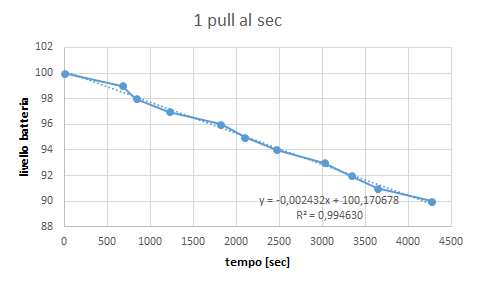
\includegraphics[width=0.75\textwidth]{1alsec.jpg} % Include the image placeholder.png
\label{fig:1 pull ogni secondo}
\end{center}

\begin{center}
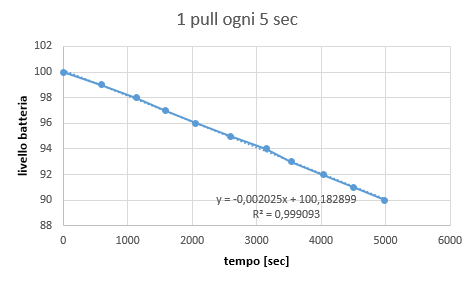
\includegraphics[width=0.75\textwidth]{5alsec.jpg} % Include the image placeholder.png
\label{fig:1 pull ogni 5 secondi}
\end{center}

\begin{center}
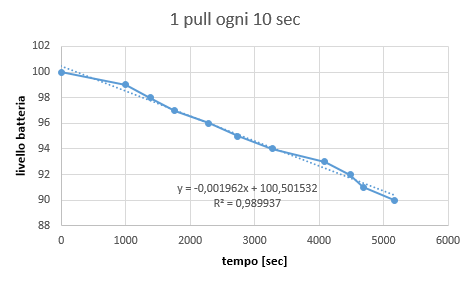
\includegraphics[width=0.75\textwidth]{10alsec.jpg} % Include the image placeholder.png
\label{fig:1 pull ogni 10 secondi}
\end{center}

\begin{center}
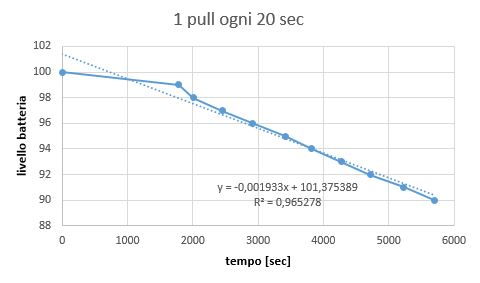
\includegraphics[width=0.75\textwidth]{20alsec.jpg} % Include the image placeholder.png
\label{fig:1 pull ogni 20 secondi}
\end{center}

%\begin{figure}[h!]
%\begin{center}
%\centering
%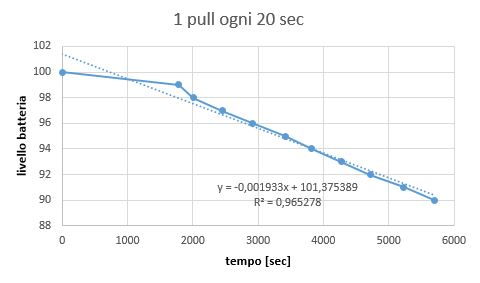
\includegraphics[width=0.85\textwidth]{20alsec.jpg} % Include the image placeholder.png
%\caption{1 pull ogni 20 secondi}
%\label{fig:1 pull ogni 20 secondi}
%\end{center}
%\end{figure}

\subsubsection{Fase 2 - \textit{Velocit\'a media di scarica} fissata la \textit{frequenza di pull}}

La stima della \textit{velocit\'a media di scarica} deriva direttamente dai modelli regressione mostrati nella precedente sezione. Avendo riscontrato una relazione di tipo lineare \'e stato possibile individuare la grandezza in questione direttamente dal coefficiente angolare dell'equazione. La seguente tabella mette in relazione la \textit{frequenza di pull} con la rispettiva \textit{velocit\'a media di scarica} della batteria:

\begin{center} \begin{table}[h] \centering \begin{tabular}{cc} \textit{p} & \(\frac{df\textsubscript{p}(\textit{t})}{dt}\) \\ \hline \multicolumn{1}{|c|}{1} & \multicolumn{1}{c|}{-0,002432} \\ \hline \multicolumn{1}{|c|}{0,2} & \multicolumn{1}{c|}{-0,002025} \\ \hline \multicolumn{1}{|c|}{0,1} & \multicolumn{1}{c|}{-0,001962} \\ \hline \multicolumn{1}{|c|}{0,05} & \multicolumn{1}{c|}{-0,001933} \\ \hline \end{tabular} \caption{\textit{Velocit\'a media di scarica}} \label{my-label} \end{table} \end{center}

\subsubsection{Fase 3 - Relazione funzionale tra la \textit{velocit\'a media di scarica} e \textit{frequenza di pull}}
Dalla regressione \'e risultata una relazione di tipo lineare tra \textit{velocit\'a media di scarica} e \textit{frequenza di pull}. Infatti risulta: 

\begin{center}
\item{(\(\frac{df\textsubscript{p}(\textit{t})}{dt}\), \textit{p}) \ding{226} \textit{lineare} poich\'e \textit{R\textsuperscript{2}}\(\approx\)0.9} 
\end{center}

Nel seguente grafico si evince tale relazione funzionale:

\begin{center}
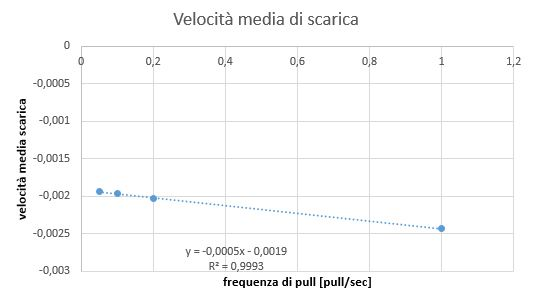
\includegraphics[width=0.75\textwidth]{veloc.jpg} % Include the image placeholder.png
\label{fig:Relazione funzionale}
\end{center}

Questo risultato \'e molto importante poich\'e dimostra che la \textit{frequenza di pull} \'e un fattore che influisce fortemente in termini di consumo energetico della batteria del dispositivo.

\section{Conclusioni e sviluppi futuri}

% Da ricordare : appendice strumenti matematici

%----------------------------------------------------------------------------------------
%	BIBLIOGRAPHY
%----------------------------------------------------------------------------------------

%\bibliographystyle{apalike}

%\bibliography{sample}

\begin{thebibliography}{1}

\bibitem{Paolo fa i pompini} Paolo \'e bello

\end{thebibliography}


\begin{appendices}
\addtocontents{toc}{\protect\setcounter{tocdepth}{2}}
\makeatletter
\addtocontents{toc}{%
  \begingroup
  \let\protect\l@chapter\protect\l@section
  \let\protect\l@section\protect\l@subsection
}
\makeatother
	
  	\section{Regressione lineare}
	
	\section{Coefficiente di determinazione}
	
\addtocontents{toc}{\endgroup}
\end{appendices}

%----------------------------------------------------------------------------------------


\end{document}